%%%%%%%%%%%%%%%%%%%%%%%%%%%%%%%%%%%%%%%%%
% TU Muenchen 17 Sommer Semester 
% Applied Reinforcement Learning
% 2nd Report 
%%%%%%%%%%%%%%%%%%%%%%%%%%%%%%%%%%%%%%%%%

%----------------------------------------------------------------------------------------
%	PACKAGES AND OTHER DOCUMENT CONFIGURATIONS
%----------------------------------------------------------------------------------------

\documentclass[a4paper, 11pt]{article} % Font size (can be 10pt, 11pt or 12pt) and paper size (remove a4paper for US letter paper)
%\usepackage{hyperref}

\usepackage[protrusion=true,expansion=true]{microtype} % Better typography
\usepackage{graphicx} % Required for including pictures
\usepackage{wrapfig} % Allows in-line images
\usepackage{booktabs}
\usepackage{mathpazo} % Use the Palatino font
\usepackage[T1]{fontenc} % Required for accented characters
\linespread{1.05} % Change line spacing here, Palatino benefits from a slight increase by default

\makeatletter
\renewcommand\@biblabel[1]{\textbf{#1.}} % Change the square brackets for each bibliography item from '[1]' to '1.'
\renewcommand{\@listI}{\itemsep=0pt} % Reduce the space between items in the itemize and enumerate environments and the bibliography

\renewcommand{\maketitle}{ % Customize the title - do not edit title and author name here, see the TITLE block below
\begin{flushright} % Right align
{\LARGE\@title} % Increase the font size of the title

\vspace{50pt} % Some vertical space between the title and author name

{\large\@author} % Author name
\\\@date % Date

\vspace{40pt} % Some vertical space between the author block and abstract
\end{flushright}
}

%----------------------------------------------------------------------------------------
%	TITLE
%----------------------------------------------------------------------------------------

\title{\textbf{Finding the Shortest Path Using Reinforcement Learning}} % Subtitle

\author{\textsc{Lingfeng Zhang, Wenhan Hao, $\&$ Tianming Qiu} % Author
\\{\textit{}}} % Institution

\date{Group: applied-rl17 / E3} % Date

%----------------------------------------------------------------------------------------

\begin{document}

\maketitle % Print the title section



%----------------------------------------------------------------------------------------
%	ESSAY BODY
%----------------------------------------------------------------------------------------

\section{Introduction of Project}
This project focuses on finding a shortest path in a map with many cross roads. The agent has to make an optimal decision to turn into a correct or best direction at each road crossing. Q learning will be adopted to train the agent.

%------------------------------------------------

\section{Markov Decision Process Description}

Obviously, the states in this model are the different road crossings. State transition, namely the transition of different road crossing, is adopted as a stochastic process. The modelling of this issue satisfies the Markov Decision Process (MDP).
 
First, it has the Markov property. And the transition from road crossing $C_{t}$ to next crossing $C_{t+1}$ is independent of all the previous states and actions. No matter which road crossing the Epuck was in or which actions it takes before the road crossing $C_{t}$, the probability that it transits from current state to next state would be never influenced. In another words, it can be represented by: $P(s_{t+1})=P(s_{t+1}|s_{t},a_{t})$. The current state captures all that is relevant about the world in order to predict what the next state will be.

Secondly, it is clear to see that the state transition is related to action. Epuck can choose to 'drive east','drive west', 'drive north' as well as 'drive south', and the consequences will be dependent on the chosen actions at current state. 

A Markov decision process is a discrete-time state transition system. It can be described formally with 5 components as a 5-tuple $(\mathcal{S,A,P}, r,\gamma)$ as below:

\textbf{$\mathcal{S}$: States} \quad First, it has a finite set of states. These states will play the role of outcomes in the decision theoretic approach, as well as providing whatever information is necessary for choosing actions. 

\textbf{$\mathcal{A}$: Action}\quad 
A small finite set includes 'drive east','drive west', 'drive north' as well as 'drive south'.

\textbf{$\mathcal{S}$: Transition probability}\quad 
The transition probabilities describe the dynamics of the world. They play the role of the next-state function in a problem-solving search, except that every state is thought to be a possible consequence of taking an action in a state. So, we specify, for each state $s_{t}$ and action $a_{t}$, the probability that the next state will be $s_{t+1}$. 
Now we just model the transition probability as the simplest one: All of them equal to one. That means if and only if Epuck takes a specific action (e.g. turn right) at the current action, it will transit into a definitely deterministic state.

\textbf{$r$: Reward}\quad  In this model we will assign a reward '+10' at the destination state and '0' at the other states. 
Also at the 'blind alley' it will get a very poor reward such as '-100'.

\textbf{$\gamma$}  \quad It is a discout factor here we select as 0.9.


%------------------------------------------------
\section{Algorithm}
In recent years, reinforcement learning has achieved many impressive results, including playing video games, and training advanced manipulation skills. The goal of this experiment is to realize artificial agents, which can be trained and can find the shortest path in intricate traffic environment. Here we consider using An off-policy TD control algorithm: Q-learning to achieve our goal.


We define a discrete-time finite-horizon discounted Markov decision process (MDP) by a tuple $(\mathcal{S,A,P}, r,\gamma)$. The agent interacts with an environment over a time of discrete time steps. At each time step, the agent receives a state from $\mathcal{S}$ and select an action from $\mathcal{A}$ according to its policy $\pi$, where $\pi$ is a mapping from states $\mathcal{S}$ to action $\mathcal{A}$. In return, the agent receives the next state and a scalar reward $r$. The process continues until the agent reaches a terminal state. The total return is the accumulated reward with discount factor $\gamma$. The action value $Q^{\pi}(s,a)$ is the expected return for selecting action a in state s and following policy $\pi$. The optimal value function $$Q^*(s,a)=\max \limits_{\pi}Q^{\pi}(S,a)$$ gives the maximum, action value for state s and action a achievable by any policy.

In Q-learning, the action value $Q(s,a)$ will be updated toward one-step return as below:$$Q(S_t,A_t)\leftarrow Q(S_t,A_t)+ \alpha [ R_{t+1} + \gamma \max \limits_{a}Q(S_{t+1},a)-Q(S_t,A_t)]$$

Each time obtaining a reward $r$ can directly affects the value of the state action pair $s,a$ that led to the reward. The pseudocode of Q-learning algorithm is shown below:
\begin{center}\textbf{Q-learning: An on-policy TD control algorithm}

\fbox{\parbox{\textwidth}{Initialize $Q(s,a)$, $\forall s \in \mathcal{S}$, $\forall a \in \mathcal{A}$, arbitrarily, and $Q($terminal-state,$\cdot)=0$

Repeat (for each episode):

\quad\quad Initialize $S$

\quad\quad Repeat (for each step of episode):

\quad\quad \quad\quad Choose $A$ from $S$ using policy derived from $Q$ (e.g., $\epsilon$-greedy)

\quad\quad \quad\quad Take action $A$, observe $R$, $S'$

\quad\quad \quad\quad $Q(S_t,A_t)\leftarrow Q(S_t,A_t)+ \alpha [ R_{t+1} + \gamma \max \limits_{a}Q(S_{t+1},a)-Q(S_t,A_t)]$

\quad\quad \quad\quad $S\leftarrow S'$

\quad\quad Until $S$ is terminal
}}

\end{center}

At each step, the agent will choose an action A according to current policy, and get the reward R. But the action value Q will be updated using another policy, here we choose the action which can maximize the next action value. That's why Q-learning is an off-policy algorithm, the policy we use to choose action and the policy we use to evaluate the value function are different. Here we prefer to the off-policy rather than on-policy algorithm, because off-policy algorithms are usually more efficient than on-policy.

\section{Simulation}
The goal of our simulation is to simulate the real traffic network. A Simulation map can be seen in Figure~\ref{fig:gallery}. The e-puck will take on a role of explorer to find the shortest path between two points of the map.

To make our tasks tractable, we consider a grid-based representation with discrete states and action. The navigational task for our mobile robots could be projected into this presentation by employing a number of actions such as 'drive east','drive west', 'drive north' as well as 'drive south' that only use a low-level controller that takes care of accelerating, moving, turning and stopping. The different crossroad in the simulated map will be considered as states. We will perform our experiment in the simulator v-rap with our test map, which has 10 states.

In reinforcement learning, the desired behavior is implicitly specified by the reward function. The goal of our reinforcement learning algorithm is to find the optimized trajectory, which can maximize the accumulated long-term reward. In our experiment, we assign a reward '+10' at the destination state and '-1' at the other states. Also at the 'blind alley' it will get a very
poor reward such as '-10' in order to let agent avoid those states.
\begin{figure}[tb]
\centering 
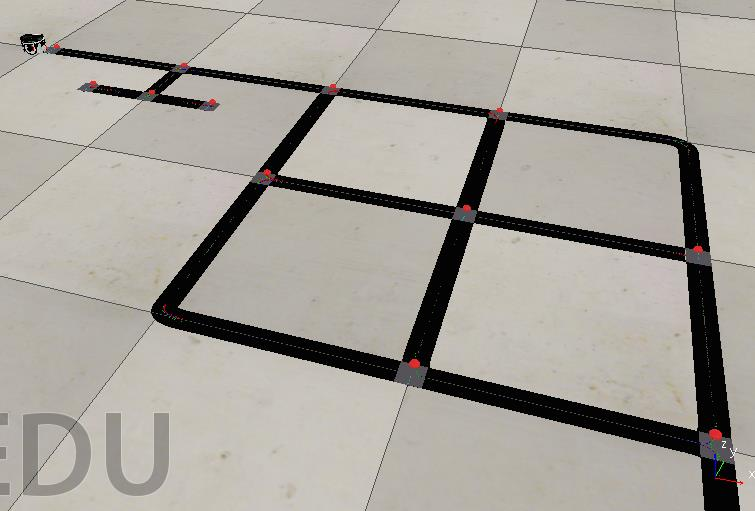
\includegraphics[width=0.9\columnwidth]{simulatemap} 
\caption[An example of a floating figure]{An example of simulation map} % The text in the square bracket is the caption for the list of figures while the text in the curly brackets is the figure caption
\label{fig:gallery} 
\end{figure}
At the begin of each simulation, two points will set up as the start point and destination, and the e-puck robot will be placed in the start point of the test map, and start to explore the test map. From one state to adjacent state, the robot will drive along the line we drawn on the ground. The under sensor on e-puck will scan the ground all the time in order to keep robot following the line and detect the label we use to distinguish state. Every time the robot reaches a new state, the Q-value will be updated with the reward we received and a new action will be selected according to the current policy. Once e-puck reaches the terminal state(destination), it will be replaced in the same start point and start a new exploration. Through trial and error, finally the action value will converge at a point, which is called optimal action value, then we can find the optimal policy for this problem.


\section{Milestones}
At present we have achieved three main Milestones: determination of the mathematical model, viable physical environment design, and successful implementation of Codes on Vrep.

First of all, the mathematical model has been determined. Before we chose the road crossing as states, and we assumed the actions as 'turn right', 'turn left' and so on. However, it caused a serious problem that the model could not satisfy Markov Property. Assume Epuck comes to a road crossing several times, first time it comes from north, namely the last state is in the north direction of current state, and second time comes from south. Since we treat this road crossing as only one state, if Epuck both choose the action 'turn right', the transition probability of the next state will be totally different and somehow dependent on not only the current state, but also the state before, like $P(s_{t+1}|s_{t},s_{t-1},a_{t})$.

Hence we choose a new set of actions as 'go east', 'go west', 'go north' and 'go south'. And on the high level of this problem we just treat our Epuck as a 'mass point'. And leave the detailed problem of action realizations to the lower level. This approach make sure the scene satisfies Markov property. 
\begin{figure}[tb]
\centering 
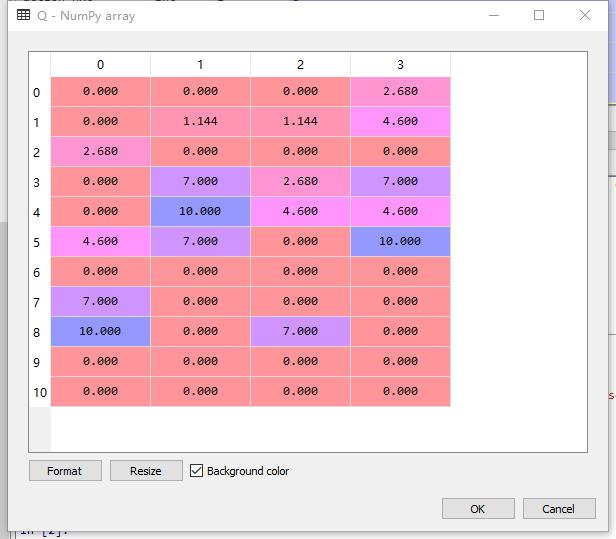
\includegraphics[width=0.5\columnwidth]{Qvalue} 
\caption[An example of a floating figure]{Q Value table after training} % The text in the square bracket is the caption for the list of figures while the text in the curly brackets is the figure caption
\label{fig:Qvalue} 
\end{figure}

Secondly, a viable simulation map has been designed on Vrep. The three floor sensors under Epuck are applied to detect the road, and the road crossings are painted with a gray color to differ from the black road and white background. Although the floor sensor are not very accurate to distinguish high resolution color space, it could be sensitive enough to detect black, white, and gray these three situations. At the moment we assume the state transition probabilities are deterministic. That means Epuck will definitely know where it will be after it takes a specific action at the current state. So we have not use other vision pattern to specify each crossing or state. This part can be improved by next stage's work. 

Thirdly the Q-learning part and the simulation execution of Epuck have been implemented on Vrep by Python. The code can be basically divided into three main parts: Q-learning algorithm, Motion or action control and perception part. Q-learning part is designed to implement a training of the finding shortest path as well as a successful and correct consequence of training. The result of training Q value table based on current simulation map is shown in Figure~\ref{fig:Qvalue}. Motion control is used for the low level control issues such as 'go east', turn a corner and so on. Perception focus on the three floor sensors to make sure Epuck could follow the line or stop correctly at the crossing roads. 

\section{Future Plan}
In the next stage we will transit the code from simulation to real epuck and set up a real road environment for Epuck. The main task is to deal with the noise in the real world and make both the training and execution more robust. We also should pay more attentions on the low level control, to make each action accurate and stable.


The detail about this project still need to be discussed, for example the probability model for state transition. Instead of deterministic it could be more accurate by defined by a mathematical model.

Also we planned to implement a few another reinforcement learning algorithms or try to use Epuck to do some other learning tasks. Based on the previous practice, the understanding of reinforcement learning could be something new.
\end{document}